

\tikzset{every picture/.style={line width=0.3pt}} %set default line width to 0.75pt        

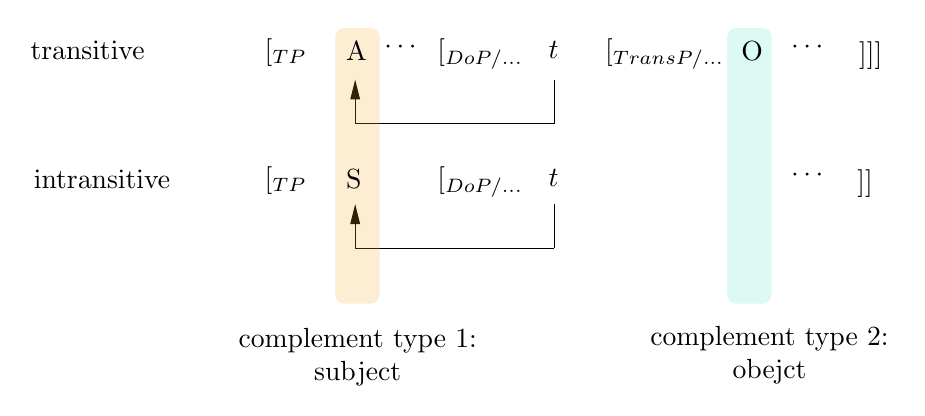
\begin{tikzpicture}[x=0.75pt,y=0.75pt,yscale=-0.8,xscale=0.8]
%uncomment if require: \path (0,418); %set diagram left start at 0, and has height of 418

%Straight Lines [id:da5607379428644168] 
\draw    (319,184.57) -- (319,160) ;
\draw [shift={(319,158)}, rotate = 90] [fill={rgb, 255:red, 0; green, 0; blue, 0 }  ][line width=0.08]  [draw opacity=0] (12,-3) -- (0,0) -- (12,3) -- cycle    ;
%Straight Lines [id:da23260332063199396] 
\draw    (439,184.57) -- (439,158) ;
%Straight Lines [id:da2641033045888783] 
\draw    (319,184.57) -- (439,184.57) ;
%Straight Lines [id:da5131301965277419] 
\draw    (319,259.57) -- (319,235) ;
\draw [shift={(319,233)}, rotate = 90] [fill={rgb, 255:red, 0; green, 0; blue, 0 }  ][line width=0.08]  [draw opacity=0] (12,-3) -- (0,0) -- (12,3) -- cycle    ;
%Straight Lines [id:da2634775648555059] 
\draw    (439,259.57) -- (439,233) ;
%Straight Lines [id:da7092937779305173] 
\draw    (319,259.57) -- (439,259.57) ;
%Rounded Rect [id:dp18336678257663852] 
\draw  [draw opacity=0][fill={rgb, 255:red, 245; green, 166; blue, 35 }  ,fill opacity=0.2 ] (307,132.34) .. controls (307,129.39) and (309.39,127) .. (312.34,127) -- (328.37,127) .. controls (331.32,127) and (333.72,129.39) .. (333.72,132.34) -- (333.72,287.59) .. controls (333.72,290.55) and (331.32,292.94) .. (328.37,292.94) -- (312.34,292.94) .. controls (309.39,292.94) and (307,290.55) .. (307,287.59) -- cycle ;
%Rounded Rect [id:dp7831208634321845] 
\draw  [draw opacity=0][fill={rgb, 255:red, 80; green, 227; blue, 194 }  ,fill opacity=0.2 ] (543,132.34) .. controls (543,129.39) and (545.39,127) .. (548.34,127) -- (564.37,127) .. controls (567.32,127) and (569.72,129.39) .. (569.72,132.34) -- (569.72,287.59) .. controls (569.72,290.55) and (567.32,292.94) .. (564.37,292.94) -- (548.34,292.94) .. controls (545.39,292.94) and (543,290.55) .. (543,287.59) -- cycle ;

% Text Node
\draw (122,133.5) node [anchor=north west][inner sep=0.75pt]   [align=left] {transitive};
% Text Node
\draw (124,210.75) node [anchor=north west][inner sep=0.75pt]   [align=left] {intransitive};
% Text Node
\draw (263,131.9) node [anchor=north west][inner sep=0.75pt]    {$[_{\text{TP}}$};
% Text Node
\draw (367,131.9) node [anchor=north west][inner sep=0.75pt]    {$[_{\text{DoP/...}}$};
% Text Node
\draw (621,133.5) node [anchor=north west][inner sep=0.75pt]   [align=left] {]]]};
% Text Node
\draw (434,133.5) node [anchor=north west][inner sep=0.75pt]   [align=left] {$\displaystyle t$};
% Text Node
\draw (550,133.5) node [anchor=north west][inner sep=0.75pt]   [align=left] {O};
% Text Node
\draw (580,133.5) node [anchor=north west][inner sep=0.75pt]   [align=left] {$\displaystyle \cdots $};
% Text Node
\draw (263,209.15) node [anchor=north west][inner sep=0.75pt]    {$[_{\text{TP}}$};
% Text Node
\draw (312,133.5) node [anchor=north west][inner sep=0.75pt]   [align=left] {A};
% Text Node
\draw (312,210.75) node [anchor=north west][inner sep=0.75pt]   [align=left] {S};
% Text Node
\draw (468,131.9) node [anchor=north west][inner sep=0.75pt]    {$[_{\text{TransP/...}}$};
% Text Node
\draw (335,133.5) node [anchor=north west][inner sep=0.75pt]   [align=left] {$\displaystyle \cdots $};
% Text Node
\draw (620,210.75) node [anchor=north west][inner sep=0.75pt]   [align=left] {]]};
% Text Node
\draw (367,209.15) node [anchor=north west][inner sep=0.75pt]    {$[_{\text{DoP/...}}$};
% Text Node
\draw (434,210.75) node [anchor=north west][inner sep=0.75pt]   [align=left] {$\displaystyle t$};
% Text Node
\draw (580,210.75) node [anchor=north west][inner sep=0.75pt]   [align=left] {$\displaystyle \cdots $};
% Text Node
\draw (320.48,306) node [anchor=north] [inner sep=0.75pt]   [align=left] {\begin{minipage}[lt]{90.41pt}\setlength\topsep{0pt}
\begin{center}
complement type 1:\\subject
\end{center}

\end{minipage}};
% Text Node
\draw (568.48,305) node [anchor=north] [inner sep=0.75pt]   [align=left] {\begin{minipage}[lt]{90.41pt}\setlength\topsep{0pt}
\begin{center}
complement type 2:\\obejct
\end{center}

\end{minipage}};


\end{tikzpicture}
